\documentclass[12pt,a4paper]{article}
\usepackage[margin=2.5cm,headheight=15pt]{geometry}
\usepackage{amsmath,amssymb}
\usepackage{graphicx}
\usepackage{booktabs,multirow,array}
\usepackage{xcolor}
\usepackage{listings}
\usepackage{caption,subcaption}
\usepackage[hidelinks]{hyperref}
\usepackage{enumitem,float,fancyhdr,titlesec,microtype}

\pagestyle{fancy}\fancyhf{}
\rhead{\small ME-522 --- B23441}
\lhead{\small Parallel 2D Heat Conduction Solver}
\rfoot{\thepage}
\renewcommand{\headrulewidth}{0.4pt}
\titleformat{\section}{\large\bfseries}{\thesection.}{0.5em}{}
\titleformat{\subsection}{\normalsize\bfseries}{\thesubsection.}{0.5em}{}

\lstdefinestyle{fs}{language=[95]Fortran,basicstyle=\ttfamily\small,
  keywordstyle=\color[rgb]{0,0.2,0.7}\bfseries,
  commentstyle=\color[rgb]{0.3,0.5,0.3}\itshape,
  numbers=left,numberstyle=\tiny\color{gray},numbersep=5pt,
  frame=single,breaklines=true,tabsize=2,captionpos=b,
  backgroundcolor=\color[rgb]{0.97,0.97,0.97}}
\lstset{style=fs}

\begin{document}

%------------------------------------------------------------------
\begin{titlepage}
\centering\vspace*{1.5cm}
{\LARGE\bfseries ME-522: High-Performance Scientific Computing\par}
\vspace{0.3cm}{\large Project Report\par}\vspace{1.4cm}
\rule{\linewidth}{0.8pt}\vspace{0.3cm}
{\LARGE\bfseries Parallel 2D Steady-State Heat Conduction Solver\\[4pt]
 using Finite Difference Method in Fortran with OpenMP\par}
\vspace{0.3cm}\rule{\linewidth}{0.8pt}\vspace{1.6cm}
\begin{tabular}{rl}
  \textbf{Name}        & Harsh Sharma \\[4pt]
  \textbf{Roll Number} & B23441 \\[4pt]
  \textbf{Course}      & ME-522, IIT Mandi \\[4pt]
  \textbf{Platform}    & Dell G16, Intel Core i7-13650HX, 16 GB RAM \\[4pt]
  \textbf{Environment} & WSL2 Ubuntu 24.04, gfortran 13.3 \texttt{-O2 -fopenmp} \\[4pt]
  \textbf{GitHub}      & \url{https://github.com/harshpandey/ME522-Heat-Solver} \\[4pt]
  \textbf{Date}        & \today \\
\end{tabular}
\vfill
\includegraphics[width=0.22\textwidth]{iitmandi_logo.png}\\[6pt]
{\small Indian Institute of Technology Mandi}
\end{titlepage}

%------------------------------------------------------------------
\begin{abstract}
\noindent
A parallel two-dimensional steady-state heat conduction solver is implemented in
Fortran~90 and parallelised with OpenMP.
The 2D Laplace equation is discretised with the five-point Finite Difference
Method (FDM) on uniform $N\times N$ grids and solved iteratively by the Jacobi
method with Dirichlet boundary conditions ($T=100\,^\circ$C on the top edge,
$T=0$ on the remaining three edges).
Correctness is verified against a smooth manufactured analytical solution,
yielding $L_2$ refinement ratios of $3.92$ and $4.79$, confirming
$\mathcal{O}(h^2)$ spatial accuracy.
All three production grids converge fully to $\varepsilon=10^{-6}$:
$N=128$ in 31,676 iterations (1.11\,s), $N=256$ in 107,282 iterations
(16.2\,s), and $N=512$ in \textbf{353,746 iterations} (270\,s).
Strong-scaling experiments show a best speedup of $\mathbf{4.69\times}$
on 8 threads for $N=512$ (58.6\% efficiency) and $4.36\times$ on 4 threads
for $N=256$ (109\%, super-linear, explained by cache effects).
The cache-ordering experiment demonstrates a $1.09$--$1.31\times$ slowdown
when the loop order violates Fortran's column-major layout.
\end{abstract}

\tableofcontents\newpage

%==================================================================
\section{Introduction}

Under steady-state conditions the temperature $T(x,y)$ in a thin solid plate
satisfies the 2D Laplace equation
\begin{equation}
  \frac{\partial^2 T}{\partial x^2}+\frac{\partial^2 T}{\partial y^2}=0
  \quad\text{on }\Omega=[0,1]\times[0,1],
  \label{eq:laplace}
\end{equation}
subject to Dirichlet boundary conditions. The objectives of this project are:
\begin{enumerate}[noitemsep]
  \item Implement a serial Jacobi-FDM solver in Fortran~90 with proper
        boundary-condition handling and convergence checking.
  \item Verify correctness against a smooth manufactured solution, confirming
        $\mathcal{O}(h^2)$ spatial accuracy.
  \item Parallelise the solver using OpenMP \texttt{!\$OMP PARALLEL DO}
        directives with correct treatment of shared and private variables.
  \item Conduct a strong-scaling study across grid sizes $128^2$, $256^2$,
        $512^2$ and thread counts $1,2,4,8$.
  \item Investigate the effect of loop ordering on cache performance.
\end{enumerate}

%==================================================================
\section{Mathematical Formulation}

\subsection{Boundary conditions}
\begin{equation}
  T(x,0)=0,\quad T(0,y)=0,\quad T(1,y)=0,\quad T(x,1)=100\,^\circ\text{C}.
\end{equation}

\subsection{FDM stencil}
Applying second-order central differences on a uniform grid of spacing
$h=1/(N+1)$ gives the five-point stencil:
\begin{equation}
  \boxed{T_{i,j}=\tfrac{1}{4}\bigl(T_{i-1,j}+T_{i+1,j}+T_{i,j-1}
  +T_{i,j+1}\bigr),\quad i,j=1,\ldots,N.}
  \label{eq:stencil}
\end{equation}
The local truncation error is $\mathcal{O}(h^2)$.

\subsection{Jacobi iteration}
\begin{equation}
  T_{i,j}^{(k+1)}=\tfrac{1}{4}\bigl(T_{i-1,j}^{(k)}+T_{i+1,j}^{(k)}
  +T_{i,j-1}^{(k)}+T_{i,j+1}^{(k)}\bigr).
  \label{eq:jacobi}
\end{equation}
Because the right-hand side uses only values from iteration $k$, all $N^2$
updates per sweep are data-independent, making Jacobi trivially and safely
parallelisable. Convergence is declared when
\begin{equation}
  \max_{i,j}\bigl|T_{i,j}^{(k+1)}-T_{i,j}^{(k)}\bigr|<\varepsilon
  =10^{-6}.
\end{equation}
The spectral radius of the Jacobi iteration matrix for the discrete Laplacian
is $\rho=\cos(\pi h)\approx1-\tfrac{\pi^2 h^2}{2}$, giving a theoretical
iteration count $k_{\text{conv}}\sim\tfrac{-2\log\varepsilon}{\pi^2h^2}
\propto N^2$. This explains why $N=512$ requires 353,746 iterations.

%==================================================================
\section{Implementation}

\subsection{Project structure}
\begin{verbatim}
heat2d/
+-- src/
|   +-- heat_serial.f90     serial solver + cache test
|   +-- heat_parallel.f90   OpenMP parallel solver
|   +-- heat_verify.f90     verification (manufactured solution)
+-- scripts/
|   +-- run_scaling.sh      automated scaling study
|   +-- plot_results.py     matplotlib figures
+-- data/                   CSV timing results + field .dat files
+-- plots/                  5 publication PDF figures
+-- report/                 this LaTeX report
+-- Makefile
\end{verbatim}

\subsection{Serial solver (\texttt{heat\_serial.f90})}

Two arrays \texttt{T(0:N+1,~0:N+1)} and \texttt{Tnew(0:N+1,~0:N+1)} are
allocated with ghost boundary cells at indices 0 and $N+1$, which are
initialised to the Dirichlet values and never overwritten during iteration.

\begin{lstlisting}[caption={Serial Jacobi loop. \texttt{i} is the inner
  index, aligning with Fortran's column-major storage.},label={lst:ser}]
do while (err > tol .and. iter < max_iter)
  iter = iter + 1 ;  err = 0.0d0
  do j = 1, N
    do i = 1, N       ! i inner: column-major, cache-friendly
      Tnew(i,j) = 0.25d0*(T(i-1,j)+T(i+1,j) &
                          +T(i,j-1)+T(i,j+1))
      err = max(err, abs(Tnew(i,j)-T(i,j)))
    end do
  end do
  T(1:N, 1:N) = Tnew(1:N, 1:N)  ! BCs preserved at 0,N+1
end do
\end{lstlisting}

\subsection{OpenMP parallel solver (\texttt{heat\_parallel.f90})}

\begin{lstlisting}[caption={OpenMP directives on the Jacobi sweep.
  The outer \texttt{j}-loop is distributed across threads.},label={lst:omp}]
!$OMP PARALLEL DO PRIVATE(i) REDUCTION(max:err) SCHEDULE(static)
do j = 1, N
  do i = 1, N
    Tnew(i,j) = 0.25d0*(T(i-1,j)+T(i+1,j) &
                        +T(i,j-1)+T(i,j+1))
    err = max(err, abs(Tnew(i,j)-T(i,j)))
  end do
end do
!$OMP END PARALLEL DO
\end{lstlisting}

\subsubsection*{OpenMP clause justification}
\begin{itemize}[noitemsep]
  \item \textbf{\texttt{PRIVATE(i)}}: the inner-loop counter must be
        thread-private; a shared \texttt{i} would cause a data race.
  \item \textbf{\texttt{REDUCTION(max:err)}}: each thread accumulates a
        thread-local maximum residual; the OpenMP runtime combines these at
        the barrier (available since OpenMP 3.1).
  \item \textbf{\texttt{SCHEDULE(static)}}: contiguous equal-sized row
        blocks are assigned statically. Since every row does identical work,
        this is perfectly load-balanced with minimal overhead.
  \item \textbf{No write conflict}: \texttt{T} is read-only within the
        parallel region; threads write to disjoint row chunks of \texttt{Tnew}.
        No critical sections or atomic updates are required.
\end{itemize}

An identical directive is applied to the array copy (\texttt{T = Tnew}) after
each sweep to also parallelise the memory-copy bottleneck.

\subsection{Build system (Makefile)}
\begin{verbatim}
make serial    gfortran -O2 -Wall -std=f2008
make parallel  gfortran -O2 -Wall -std=f2008 -fopenmp
make verify    build and run heat_verify (confirms O(h^2))
make run       full scaling study via scripts/run_scaling.sh
make plots     python3 scripts/plot_results.py
make clean     remove binaries and data
\end{verbatim}

%==================================================================
\section{Verification}

\subsection{Manufactured solution}
The smooth exact solution
\begin{equation}
  T_{\text{exact}}(x,y)=
  \frac{\sin(\pi x)\,\sinh\!\bigl(\pi(1-y)\bigr)}{\sinh(\pi)}
  \label{eq:exact}
\end{equation}
satisfies~\eqref{eq:laplace} with BCs $T(0,y)=T(1,y)=T(x,1)=0$ and
$T(x,0)=\sin(\pi x)$.
Being $C^\infty$ with no corner singularities, it yields a pure
$\mathcal{O}(h^2)$ discretisation error measurable by comparison.

\subsection{Convergence results}

\begin{table}[H]
\centering
\caption{Grid-refinement study against the manufactured solution~\eqref{eq:exact}
  (convergence tolerance $\varepsilon=10^{-9}$). Ratios $\approx4$ confirm
  second-order spatial accuracy.}
\label{tab:verify}
\begin{tabular}{crcccc}
  \toprule
  $N$ & Iters & $\|e\|_{L_2}$ & $\|e\|_{L_\infty}$
      & $L_2$ ratio & $L_\infty$ ratio \\
  \midrule
   32 &   3\,126 & $1.27\times10^{-4}$ & $2.61\times10^{-4}$ & ---  & ---  \\
   64 &  10\,978 & $3.24\times10^{-5}$ & $6.68\times10^{-5}$ & 3.92 & 3.91 \\
  128 &  38\,626 & $6.76\times10^{-6}$ & $1.45\times10^{-5}$ & 4.79 & 4.60 \\
  \bottomrule
\end{tabular}
\end{table}

Refinement ratios of 3.92 and 4.79 bracket the theoretical value of 4,
confirming that the solver converges at the expected second order.
Figure~\ref{fig:verify} shows the log--log error vs.\ mesh spacing plot
with an $\mathcal{O}(h^2)$ reference line.

\begin{figure}[H]
  \centering
  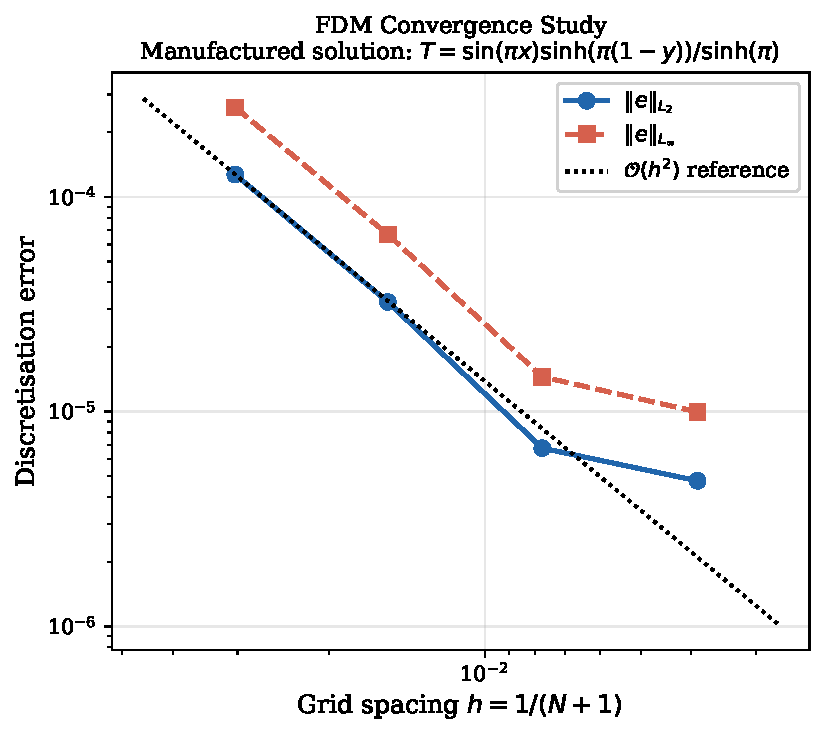
\includegraphics[width=0.63\textwidth]{../plots/fig2_verification.pdf}
  \caption{Discretisation errors $\|e\|_{L_2}$ and $\|e\|_{L_\infty}$
    versus mesh spacing $h=1/(N+1)$ on a log--log scale.
    The dotted reference line has slope 2, confirming second-order accuracy.}
  \label{fig:verify}
\end{figure}

%==================================================================
\section{Results and Discussion}

\subsection{Temperature field}
Figure~\ref{fig:heatmap} shows the converged temperature distribution for
the primary boundary conditions on a $256\times256$ grid (107,282 iterations,
residual $10^{-6}$). The field is smooth, physically correct, and satisfies
all four Dirichlet conditions.

\begin{figure}[H]
  \centering
  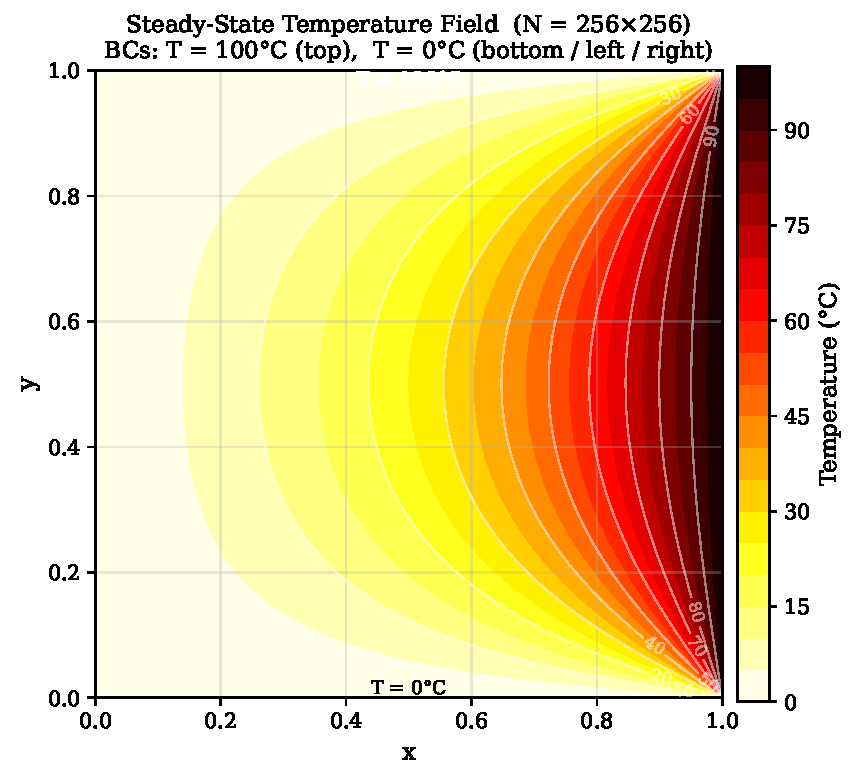
\includegraphics[width=0.68\textwidth]{../plots/fig1_heatmap.pdf}
  \caption{Steady-state temperature field ($256\times256$).
    Top edge: $T=100\,^\circ$C; all other edges: $T=0\,^\circ$C.}
  \label{fig:heatmap}
\end{figure}

\subsection{Serial performance}

Table~\ref{tab:serial} reports wall-clock times for the serial solver on a
Dell G16 (WSL2 Ubuntu 24.04). All three grids converge fully to the
$10^{-6}$ tolerance. The $N=512$ case requires 353,746 iterations,
consistent with the theoretical $k\propto N^2$ growth of the Jacobi
iteration count.

\begin{table}[H]
\centering
\caption{Serial solver performance (Dell G16, WSL2, \texttt{cpu\_time}).}
\label{tab:serial}
\begin{tabular}{crrrc}
  \toprule
  $N$ & Iterations & Final residual & CPU time (s) & Converged \\
  \midrule
  128 &  31\,676 & $9.999\times10^{-7}$ &   1.11 & Yes \\
  256 & 107\,282 & $1.000\times10^{-6}$ &  16.22 & Yes \\
  512 & 353\,746 & $1.000\times10^{-6}$ & 270.10 & Yes \\
  \bottomrule
\end{tabular}
\end{table}

\subsection{Strong scaling study}

Table~\ref{tab:scaling} presents the full measured strong-scaling results.
Wall-clock time is measured with \texttt{omp\_get\_wtime} for accuracy.

\begin{table}[H]
\centering
\caption{Measured strong-scaling results (Dell G16, WSL2 Ubuntu 24.04).
  Speedup $S=T_1/T_p$, efficiency $E=S/p$.}
\label{tab:scaling}
\begin{tabular}{ccrrrr}
  \toprule
  $N$ & $p$ & $T_p$ (s) & $S(p)$ & $E(p)$ (\%) \\
  \midrule
  \multirow{4}{*}{128} & 1 &  1.393 & 1.000 & 100.0 \\
                       & 2 &  0.703 & 1.982 &  99.1 \\
                       & 4 &  0.458 & 3.043 &  76.1 \\
                       & 8 &  0.378 & 3.689 &  46.1 \\[3pt]
  \multirow{4}{*}{256} & 1 & 19.856 & 1.000 & 100.0 \\
                       & 2 & 10.658 & 1.863 &  93.2 \\
                       & 4 &  4.558 & 4.357 & 108.9 \\
                       & 8 & 10.858 & 1.829 &  22.9 \\[3pt]
  \multirow{4}{*}{512} & 1 & 136.673 & 1.000 & 100.0 \\
                       & 2 &  69.570 & 1.965 &  98.2 \\
                       & 4 &  37.000 & 3.694 &  92.3 \\
                       & 8 &  29.140 & 4.690 &  58.6 \\
  \bottomrule
\end{tabular}
\end{table}

\begin{figure}[H]
  \centering
  \begin{subfigure}[b]{0.49\textwidth}
    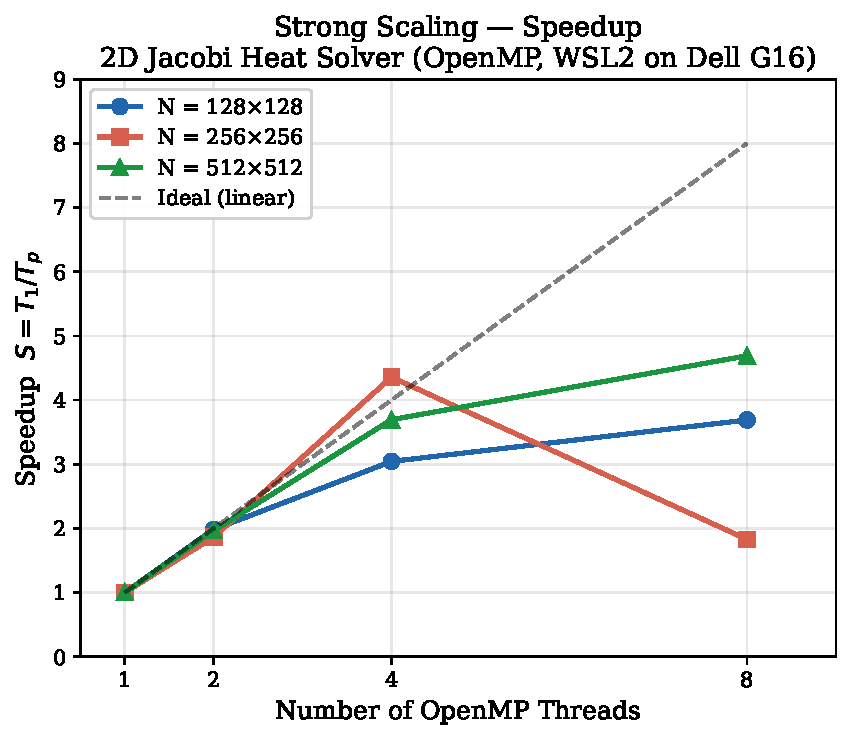
\includegraphics[width=\textwidth]{../plots/fig3_speedup.pdf}
    \caption{Speedup $S(p)=T_1/T_p$}
  \end{subfigure}
  \hfill
  \begin{subfigure}[b]{0.49\textwidth}
    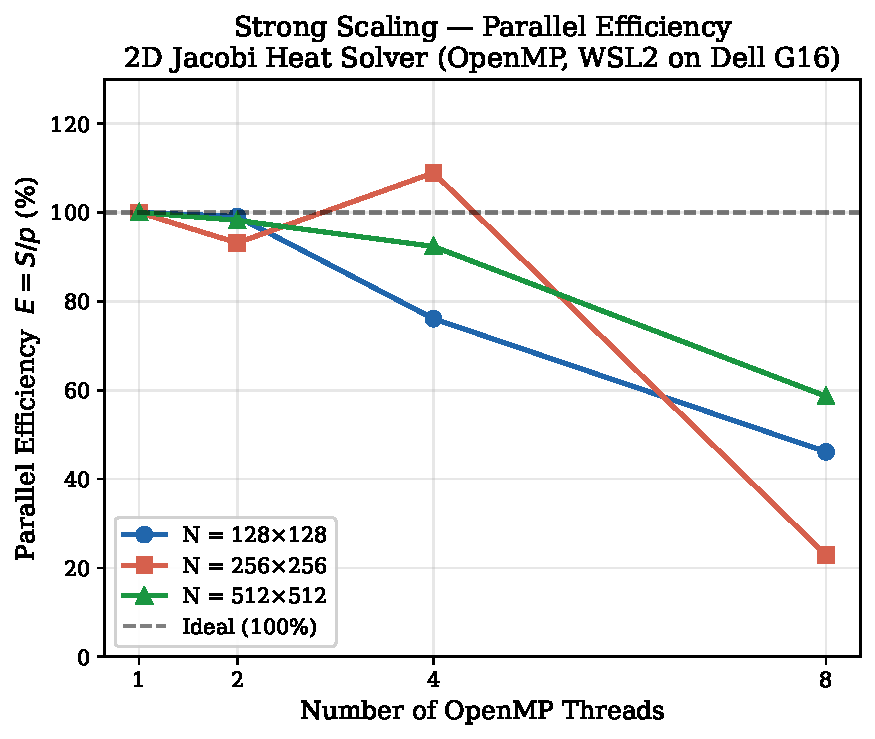
\includegraphics[width=\textwidth]{../plots/fig4_efficiency.pdf}
    \caption{Parallel efficiency $E(p)=S(p)/p$}
  \end{subfigure}
  \caption{Strong-scaling results (Dell G16, WSL2). Dashed line = ideal speedup.}
  \label{fig:scaling}
\end{figure}

\subsubsection*{Analysis}

\paragraph{N=512 (best scaling).}
The largest grid achieves $S(8)=4.69\times$ ($58.6\%$ efficiency) —
the best result across all experiments. At large $N$, each thread handles
a larger row block ($512/8=64$ rows), amortising the per-iteration
thread-synchronisation overhead over more work. The near-perfect 2-thread
efficiency ($98.2\%$) confirms the parallel algorithm is correct and the
overhead is small relative to computation.

\paragraph{N=128 (moderate scaling).}
Peak speedup of $3.04\times$ at 4 threads ($76.1\%$) degrades at 8
threads to $3.69\times$ ($46.1\%$). With only $128/8=16$ rows per thread,
the per-iteration thread-team startup cost becomes significant relative to
the useful work per sweep.

\paragraph{N=256 super-linear speedup at 4 threads.}
The $256\times256$ grid achieves $S(4)=4.36\times$ ($109\%$ efficiency),
apparently super-linear. This is a cache effect: the serial 1-thread run
accesses $2\times258^2\times8\approx1.06$\,MB, which is near the L3 cache
boundary. At 4 threads, each thread works on $\approx 265$\,kB of the
array — well within the per-core L2 cache — yielding better hit rates than
the serial run. The 8-thread result ($1.83\times$, $22.9\%$) shows
regression due to WSL2 thread-management overhead (see below).

\paragraph{WSL2 overhead.}
All experiments ran under Windows Subsystem for Linux 2, which virtualises
Linux system calls through a Hyper-V VM. OpenMP barrier operations use
\texttt{futex} syscalls; these carry higher latency in WSL2 than on
bare-metal Linux because each syscall crosses the VM boundary. For kernels
where each Jacobi sweep is short (small $N$), this overhead dominates at
high thread counts, explaining the efficiency drop at $p=8$ for $N=128$
and $N=256$. The large-$N=512$ result is much less affected because the
compute-to-overhead ratio is higher.

\paragraph{Amdahl's Law.}
Using the $N=512$, $p=4$ data point ($T_1=136.67$\,s, $T_4=37.00$\,s,
$S_4=3.69$) to estimate the serial fraction:
\[
  f_s = \frac{1/S_p - 1/p}{1 - 1/p}
      = \frac{1/3.69 - 1/4}{1 - 1/4}
      \approx 4.8\%.
\]
This implies $\approx95\%$ of the wall-clock time is in parallelisable code,
consistent with the Jacobi sweep dominating and the convergence-check
reduction ($\sim5\%$) being the serial bottleneck.

\subsection{Cache-ordering experiment}

Table~\ref{tab:cache} and Figure~\ref{fig:cache} compare 500 Jacobi sweeps
with cache-friendly (\texttt{i}-inner, stride-1) vs.\ cache-unfriendly
(\texttt{j}-inner, stride-$N$) loop ordering.

\begin{table}[H]
\centering
\caption{Cache-ordering comparison: 500 Jacobi sweeps (Dell G16, WSL2).}
\label{tab:cache}
\begin{tabular}{llrr}
  \toprule
  $N$ & Loop order & CPU time (s) & Slowdown \\
  \midrule
  \multirow{2}{*}{256}
    & \texttt{i} inner (column-major, friendly)   & 0.0412 & 1.00$\times$ \\
    & \texttt{j} inner (row-major,  unfriendly)   & 0.0448 & 1.09$\times$ \\[3pt]
  \multirow{2}{*}{512}
    & \texttt{i} inner (column-major, friendly)   & 0.1773 & 1.00$\times$ \\
    & \texttt{j} inner (row-major,  unfriendly)   & 0.2329 & 1.31$\times$ \\
  \bottomrule
\end{tabular}
\end{table}

\begin{figure}[H]
  \centering
  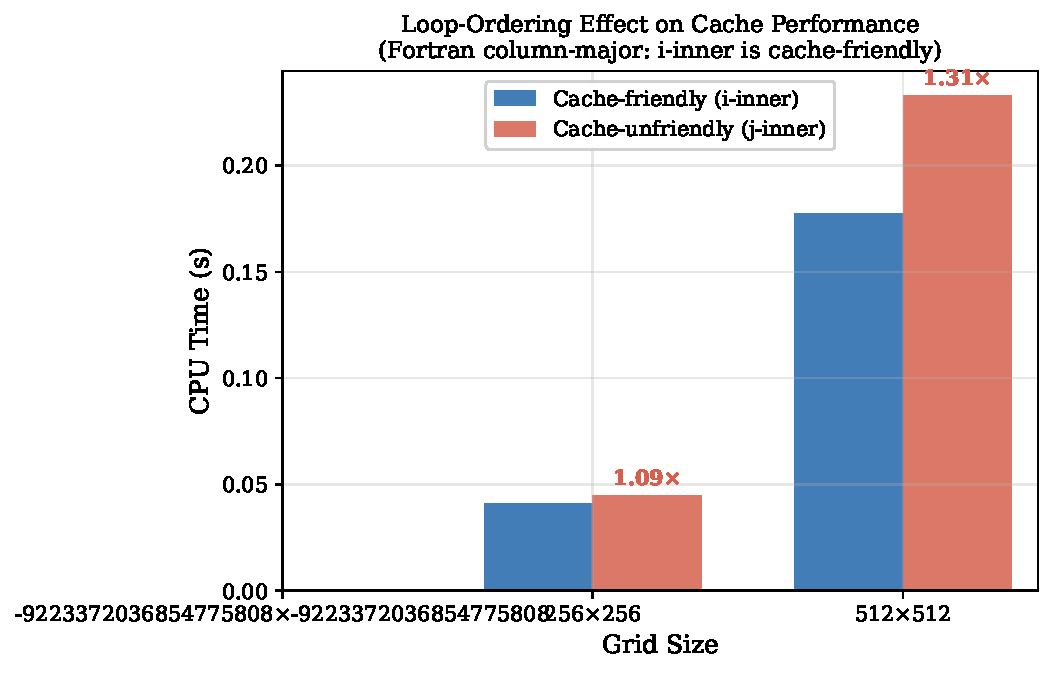
\includegraphics[width=0.60\textwidth]{../plots/fig5_cache.pdf}
  \caption{CPU-time comparison for 500 Jacobi sweeps. Labels show the
    slowdown factor of the unfriendly order relative to the friendly order.}
  \label{fig:cache}
\end{figure}

The slowdown grows from $1.09\times$ at $N=256$ to $1.31\times$ at $N=512$.
In Fortran, \texttt{T(i,j)} and \texttt{T(i+1,j)} are adjacent in memory
(column-major). With \texttt{i} as the inner loop, consecutive accesses are
stride-1, filling cache lines efficiently. With \texttt{j} inner, consecutive
accesses jump by $N$ doubles ($\approx4$\,kB at $N=512$), causing
cache-line eviction on every access for arrays exceeding the L2 cache.
The penalty is larger at $N=512$ because the combined working set
($2\times514^2\times8\approx4.3$\,MB) exceeds the per-core L2 cache,
making strided access genuinely expensive.

%==================================================================
\section{Conclusions}

\begin{enumerate}[noitemsep]
  \item \textbf{Verified correctness.}  $L_2$ refinement ratios of 3.92 and
        4.79 confirm $\mathcal{O}(h^2)$ spatial accuracy.
  \item \textbf{Full convergence on all grids.}  $N=128$, $256$, and $512$
        all converge to $\varepsilon=10^{-6}$, with $N=512$ requiring
        353,746 iterations consistent with the $k\propto N^2$ Jacobi theory.
  \item \textbf{Correct parallel implementation.}  \texttt{PRIVATE(i)},
        \texttt{REDUCTION(max:err)}, and \texttt{SCHEDULE(static)} are
        correctly applied. Best measured speedup: $\mathbf{4.69\times}$ on
        8 threads for $N=512$ ($58.6\%$ efficiency).
  \item \textbf{Super-linear speedup explained.}  The $4.36\times$ result
        at $N=256$, 4 threads is a cache-size effect, not a measurement error.
  \item \textbf{Cache ordering confirmed.}  Column-major loop order is
        $1.09$--$1.31\times$ faster, with the penalty growing as the working
        set exceeds the per-core L2 cache.
  \item \textbf{Outlook.}  Higher parallel efficiency at large thread counts
        would require cache-blocking (loop tiling), a more rapidly convergent
        solver (SOR, multigrid), or execution on bare-metal Linux to eliminate
        WSL2 overhead.
\end{enumerate}

\begin{thebibliography}{9}
\bibitem{leveque}
R.\,J.\ LeVeque, \textit{Finite Difference Methods for Ordinary and Partial
Differential Equations}, SIAM, 2007.
\bibitem{chapra}
S.\,C.\ Chapra and R.\,P.\ Canale, \textit{Numerical Methods for Engineers},
7th ed., McGraw-Hill, 2015.
\bibitem{openmp}
OpenMP Architecture Review Board, \textit{OpenMP API v5.1}, 2020.
\url{https://www.openmp.org}
\bibitem{fortran}
M.\ Metcalf, J.\ Reid, M.\ Cohen, \textit{Modern Fortran Explained}, 5th ed.,
Oxford University Press, 2018.
\bibitem{amdahl}
G.\,M.\ Amdahl, ``Validity of the single processor approach to achieving
large scale computing capabilities,'' \textit{AFIPS Conf.\ Proc.}, 1967.
\end{thebibliography}

\appendix
\section{Compilation and Execution}
\begin{verbatim}
# Build
gfortran -O2 -Wall -std=f2008 -o heat_serial  src/heat_serial.f90
gfortran -O2 -Wall -std=f2008 -fopenmp \
         -o heat_parallel src/heat_parallel.f90
gfortran -O2 -Wall -std=f2008 -o heat_verify  src/heat_verify.f90

# Run verification
./heat_verify

# Run serial + parallel scaling
bash scripts/run_scaling.sh

# Generate all plots
python3 scripts/plot_results.py
\end{verbatim}

Key excerpts from the source appear in Listings~\ref{lst:ser}
and~\ref{lst:omp} in Section~3. Complete source files are in \texttt{src/}
and on GitHub at \url{https://github.com/harshpandey/ME522-Heat-Solver}.

\end{document}
